\documentclass[15pt,a5paper,reqno]{article}
\usepackage{hyperref}
\usepackage[warn]{mathtext}
\usepackage[utf8]{inputenc}
\usepackage[T2A]{fontenc}
\usepackage[russian]{babel}
\usepackage{amssymb, amsmath, multicol}
\usepackage{graphicx}
\usepackage[shortcuts,cyremdash]{extdash}
\usepackage{wrapfig}
\usepackage{floatflt}
\usepackage{lipsum}
\usepackage{verbatim}
\usepackage{concmath}
\usepackage{euler}
\usepackage{xcolor}
\usepackage{etoolbox}
\usepackage{fancyhdr}
\usepackage{subfiles}
\usepackage{enumitem}
\usepackage{amsthm}
\usepackage{indentfirst}
\usepackage{import}
\usepackage{tabto}

\DeclareMathOperator{\sign}{sign}

\RequirePackage[ left     = 1.5cm,
  right    = 1.5cm,
  top      = 2.0cm,
  bottom   = 1.25cm,
  includefoot,
  footskip = 1.25cm ]{geometry}
\setlength    {\parskip}        { .5em plus .15em minus .08em }
%\setlength    {\parindent}      { .0em }
\renewcommand {\baselinestretch}{ 1.07 }

\fancyhf{}

\renewcommand{\footrulewidth}{ .0em }
\fancyfoot[C]{\texttt{\textemdash~\thepage~\textemdash}}

\makeatletter
\patchcmd\l@section{%
  \nobreak\hfil\nobreak
}{%
  \nobreak
  \leaders\hbox{%
    $\m@th \mkern \@dotsep mu\hbox{.}\mkern \@dotsep mu$%
  }%
  \hfill
  \nobreak
}{}{\errmessage{\noexpand\l@section could not be patched}}
\makeatother
\parindent = 1cm % отступ при красной строке⏎
\pagestyle{fancy}    
\renewcommand\qedsymbol{$\blacksquare$}

\newcommand{\when}[2]{
  \left. #1 \right|_{#2} \hspace
}
\renewcommand{\kappa}{\varkappa}
\RequirePackage{caption2}
\renewcommand\captionlabeldelim{}
\newcommand*{\hm}[1]{#1\nobreak\discretionary{}

\DeclareSymbolFont{T2Aletters}{T2A}{cmr}{m}{it}
{\hbox{$\mathsurround=0pt #1$}}{}}
% Цвета для гиперссылок
\definecolor{linkcolor}{HTML}{000000} % цвет ссылок
\definecolor{urlcolor}{HTML}{799B03} % цвет гиперссылок
 
\hypersetup{pdfstartview=FitH,  linkcolor=linkcolor,urlcolor=urlcolor, colorlinks=true}


%\setcounter{secnum[utf8x]depth}{0}

\begin{document}

% НАЧАЛО ТИТУЛЬНОГО ЛИСТА
\begin{center}
  {\small ФЕДЕРАЛЬНОЕ ГОСУДАРСТВЕННОЕ АВТОНОМНОЕ ОБРАЗОВАТЕЛЬНОЕ\\ УЧРЕЖДЕНИЕ ВЫСШЕГО ОБРАЗОВАНИЯ\\ МОСКОВСКИЙ ФИЗИКО-ТЕХНИЧЕСКИЙ ИНСТИТУТ\\ (НАЦИОНАЛЬНЫЙ ИССЛЕДОВАТЕЛЬСКИЙ УНИВЕРСИТЕТ)\\ ФИЗТЕХ-ШКОЛА РАДИОТЕХНИКИ И КОМПЬЮТЕРНЫХ ТЕХНОЛОГИЙ}\\
  \hfill \break
  \hfill \break
  \hfill \break
  \Huge{Работа 2.3.1. Получение и измерение вакуума}\\
\end{center}

\hfill \break
\hfill \break
\hfill \break
\hfill \break
\hfill \break
\hfill \break

\begin{flushright}
  \normalsize{Работу выполнил:}\\
  \normalsize{\textbf{Долгов Александр Алексеевич, группа Б01-106}}\\
\end{flushright}

\hfill \break
\hfill \break
\hfill \break

\begin{center}
  \normalsize{\textbf{Долгопрудный, 2022}}
\end{center}


\thispagestyle{empty} % выключаем отображение номера для этой страницы

% КОНЕЦ ТИТУЛЬНОГО ЛИСТА

\newpage
\thispagestyle{plain}
\tableofcontents
\thispagestyle{plain}
\newpage

\section{Аннотация}

	В данной работе исследуются некоторые свойства вакуума, полученного с помощью вакуумного насоса. Измеряется объём форвакуумной и высоковакуумной частей установки, а также определяются скорости откачки системы при различных состояниях вакуума.

\section{Теоретические сведения}

    Введём основные термины, используемые в данной работе.
    
    \textbf{Вакуум} - такое состояние газа, при котором длина свободного пробега его молекул по порядку величины сравнима с характерным линейным размером сосуда.
    
    \textbf{Быстрота откачивающего действия (скорость откачки) вакуумной системы} (S) - объём газа, проходящего через рассматриваемое сечение вакуумпровода в единицу времени при текущем давлении в данном сечении.
    
    \begin{equation}
        S = \frac{dV}{dt},\>\>\>[S] = \frac{\text{м}^3}{\text{с}}
    \end{equation}
    
    \textbf{Пропускная способность (проводимость)} (U) - отношение потока газа через вакуумпровод к разность давлений в откачиваемом объёме и на входе в насос.
    
    \begin{equation}\label{conductivity}
        U = \frac{Q}{P_1 - P_2},\>\>\>[U] = \frac{\text{м}^3}{\text{с}},
    \end{equation}
    где $P_1$ - давление в откачиваемом объёме, $P_2$ - давление на входе в насос, $Q$ - поток газа через вакуумпровод с соответствующими давлениями на концах.
    
    Ясно, что в процессе откачки давление меняется как во времени, так и вдоль вакуумпровода. Однако через некоторое время, зависящее от параметров системы) течение разреженного газа переходит в квазистационарный режим, в котором поток газа становится практически постоянным и равным количеству газа, поступающего в систему в единицу времени вследствие наличия течей. Для такого режима справедливо уравнение непрерывности:
    
    \begin{equation}\label{continuity}
        P_1S_1 = P_2S_2 = Q
    \end{equation}
    
    \noindentПолучим основное уравнение вакуумной техники. Из \eqref{conductivity} и \eqref{continuity}:
    \[U = \frac{Q}{P_1 - P_2} = \frac{Q}{\frac{Q}{S_1} - \frac{Q}{S_2}} = \frac{1}{\frac{1}{S_1} - \frac{1}{S_2}}\]
    
    \begin{equation}\label{main}
        \frac{1}{S_1} = \frac{1}{S_2} + \frac{1}{U}
    \end{equation}
    
    Возникновение течей количественно характеризуется величиной, которая называется натекание.
    
    \textbf{Натекание} ($Q_{out}$) - быстрота изменения давления в данном объёме при отключенных средствах откачки.
    
    \begin{equation}\label{leak}
        Q_{out} = V\frac{dP}{dt}
    \end{equation}
    
    Допустимым считается такое натекание, что $Q_{out} \ll Q$
    
    \noindent\underline{Режимы течения газа}:
    
    Для классификации режимов течения применяется число Кнудсена ($Kn = \frac{\lambda}{d}$), равное отношению длины свободного пробега молекулы газа к характерному линейному размеру сосуда.
    
    Если $Kn \ll 1$, то течение называется гидродинамическим (вязкостным); молекулы сталкиваются преимущественно друг с другом. Если $Kn \gg 1$, то течение называется молекулярным (кнудсеновским); молекулы сталкиваются преимущественно со стенками сосуда. Если $Kn \approx
    1$, то в системе могут существовать оба описанных вида течения.
    
    \noindent\underline{Проводимость отверстия в стенке}:
    
    Далее индекс 1 относится к величинам с одной стороны от стенки, 2 - с другой.
    Пусть $\nu$ - число молекул, пролетающих через единицу площади отверстия за единицу времени, $A$ - площадь отверстия, $n$ - концентрация молекул, $v$ - средняя скорость молекул, тогда справедливы соотношения:
    
    \noindent1) Из определения:
     
    \begin{eqnarray}\label{definition}
        \nu = \frac{1}{A}\left(\frac{dN_2}{dt} - \frac{dN_1}{dt}\right) = \frac{1}{A}\left(\frac{d(n_2V)}{dt} - \frac{d(n_1V)}{dt}\right) = \nonumber\\
        = \frac{n_2 - n_1}{A}\frac{dV}{dt} = \frac{1}{AkT}(P_2 - P_1)U_{\text{отв}}
    \end{eqnarray}
    
    \noindent2) Из анализа движения молекул
    
    \begin{equation}\label{movement}
        \nu = \nu_1 - \nu_2 = \frac{1}{4}n_2v - \frac{1}{4}n_1v = \frac{1}{4}v(n_1 - n_2) = \frac{1}{4}\frac{v}{kT}(P_2 - P_1)
    \end{equation}
    
    Из уравнений \eqref{definition} и \eqref{movement} получаем выражение для проводимости отверстия:
    
    \begin{equation}
        U_{\text{отв}} = \frac{1}{4}Av = \frac{1}{4}\pi R^2 \sqrt{\frac{8kT}{\pi m}}
    \end{equation}
    
    \noindent\underline{Проводимость длинного трубопровода}:
    
    Будем рассматривать длинный трубопровод, то есть такой, что $L \gg\\\gg R $, где $L$ - длина трубопровода, $R$ - его радиус.
    
    В случае гидродинамического режима откачки проводимость получается из формулы Пуазёйля:
    
    \begin{equation}
        U_{\text{тр}} = \frac{\pi R^4}{8\eta L}\Delta P,
    \end{equation}
    где $\Delta P$ - перепад давления вдоль трубы, $\eta$ - вязкость газа.
    
    В случае молекулярного режима откачки выражение для проводимости имеет вид:
    
    \begin{equation}
        U_{\text{тр}} = \frac{4}{3}\frac{R^3}{L}\sqrt{\frac{2\pi kT}{m}},
    \end{equation}
    где $m$ - масса молекулы газа.
    
    \noindent\underline{Время откачки}:
    
    Пусть в начальный момент времени в откачиваемом объёме $V_0$ было давление $P$. Пусть также за время $dt$ это давление изменилось на $dP$. Тогда верно соотношение: $S_0Pdt = -V_0dP$, которое можно записать в виде
    
    \begin{equation}
        dt = \frac{V_0}{S_1}\frac{dP}{P}
    \end{equation}
    
    С учётом уравнение \eqref{main} получаем:
    
    \begin{equation}\label{time}
        dt = -V_0\left(\frac{1}{S_2} + \frac{1}{U}\right)\frac{dP}{P}
    \end{equation}
    
    В общем случае для решения \eqref{time} нужно знать зависимость $S_2$ от давления. Если же $S_2 = const$, то решение имеет вид:
    
    \begin{equation}
        P(t) = P_1\cdot exp\left(-\frac{S_0}{V_0}t\right)
    \end{equation}
    
\section{Экспериментальная установка}

    В данной работе применяются два вида насосов: мембранный (диафрагменный) и турбомолекулярный. Мембранный насос обладает низкой скоростью откачки, и с его помощью возможно получить лишь средний вакуум. Турбомолекулярный насос позволяет получить высокий вакуум.
     
    Для измерения давления используются два вакуумметра: терморезисторный (вакуумметр Пирани) и магнетронный (с холодным катодом). Вакуумметр Пирани не применим в области низкого вакуума, так как его принцип действия основан на зависимости теплопроводности газа от давления, но при давлении менее $10^{-3}$ Торр теплопроводность становится постоянной. Магнетронный вакуумметр работает в условиях высокого и сверхвысокого вакуума, однако его не рекомендовано применять для исследования среднего вакуума, поскольку материал катода распыляется потоком ионов газа.
    
    \noindentСхема экспериментальной установки приведена на рисунке 1.
    \begin{figure}[h]
		\centering
		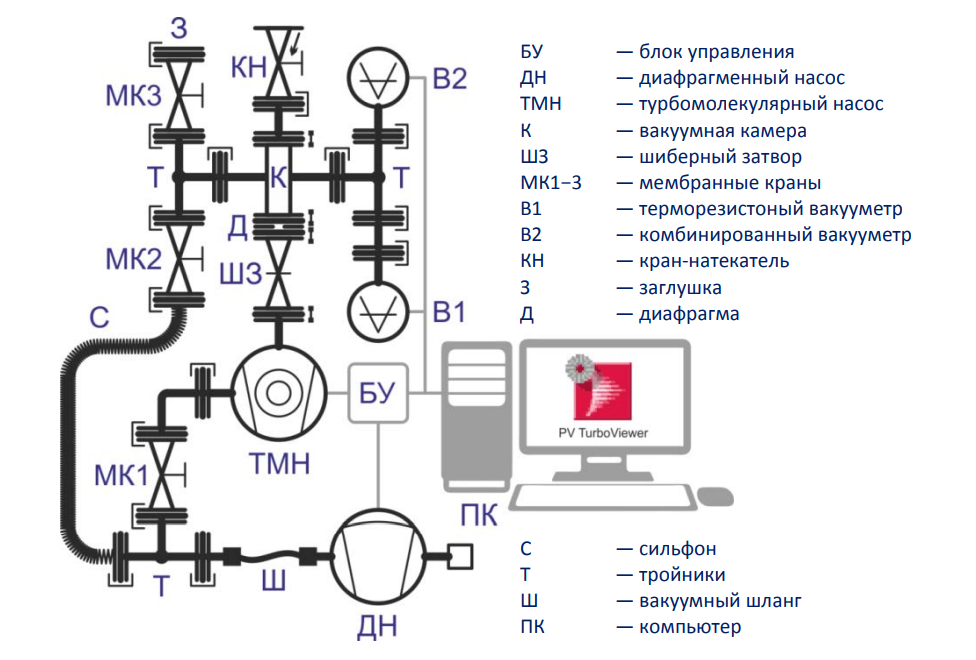
\includegraphics[width=11cm]{Установка.PNG}
		\caption{Схема экспериментальной установки}
		\label{stand}
	\end{figure}
	
	Управление основными функциями установки осуществляется с помощью программного обеспечения PV TurboViewer. Откачка вакуммной камеры может производиться как двумя насосами через шиберный затвор, так и только диафрагменным насосом по пути: сильфон $\rightarrow$ мембранный кран 2 $\rightarrow$ тройник $\rightarrow$ шланг. Для измерения давления используются цифровой терморезисторный вакуумметр PPT 100 и комбинированный вауумметр MPT 100 (одновременно терморезисторный и магнетронный). 
	
\section{Методика измерений}
    
    \subsection{Определение полного объёма установки}
    
    К откачанной установке был подключен сильфон, заполненный воздухом при атмосферном давлении. Объём сильфона равен $V_c$.
    
    Далее был открыт кран МК3, вследствие чего воздух из сильфона распространился по всей установке и занял объём $V_{\text{уст}} + V_c$. Такое расширение является неравновесным процессом, однако внутренняя энергия газа остаётся постоянной в предположении, что установка является адиабатической оболочной. Таким образом, для газа в двух состояния справедлив закон Бойля-Мариотта:
    
    \begin{equation}
        P_{\text{атм}}V_c = P_2(V_{\text{уст}} + V_c),
    \end{equation}
    где $P_{\text{атм}}$ -  атмосферное давление, $P_2$ - установившееся давление во всей установке. 
    
    \noindentОтсюда получаем:
    \begin{equation}
        V_{\text{уст}} = V_c\frac{P_{\text{атм}} - P_2}{P_2}
    \end{equation}
    
    \subsection{Измерение скорости откачки форвауумным и турбомолекулярным насосами}
     
    Установка была заполнена воздухом при атмосферном давлении, а затем откачивалась форвакуумным насосом до тех пор, пока давление в системе не перестало меняться с точностью до возникающих флуктуаций. По зависимости $P(t)$ можно получить величину $\frac{S_0}{V_{\text{уст}}}$, откуда уже найти $S_0$.
    
    В случае откачки турбомолекулярным насосом величина $S_0$ получается идентично.
    
    \subsection{Определение уровня течей}
    Для оценки уровня течей после остановки откачки турбомолекулярным насосом измерялось давление в системе с помощью вакуумметра В2. По полученной зависимости, используя формулу \eqref{leak}, можно определить величину натекания.
    
\section{Обработка результатов измерений}

    \subsection{Определение полного объёма установки}
    
    Объём сильфона: $V_{c} = 265\text{ мл}$ (погрешность считаем равной нулю, так как данные получены непосредственно из текста методического пособия).
    Измерение атмосферного давления не производилось, поэтому считаем, что $P_{\text{атм}} = 760\text{ Торр}$.
    Давление в системе, измеренное с помощью вакуумметра В1 будем обозначать $P_1$, с помощью В2 - $P_2$.
    
    \noindentПосле откачки объёма установки:
    
    $P_1 = 3,7\text{ мбар}$;
    
    $P_2 = 3,9\text{ мбар}$.
    
    Заметим, что эти величины на 3 порядка меньше атмосферного давления, то есть давления воздуха в сильфоне. Поэтому этим давлением можно пренебречь и считать, что воздух из сильфона расширяется в вакуум.
    
    \noindentПосле распространения воздуха в форвакуумную камеру:
    
    $P_1 = 0,18\text{ бар}$;
    
    $P_2 = 1\text{ бар}$.
    
    \noindentБолее корректно давление измерено вакуумметром PPT 100, так как в силу своей конструкции он больше подходит для измерения высокого и среднего вакуума, в то время как MPT 100 более точен в области низкого вакуума. Отсюда получаем:
    
    $V_{\text{фвк}} = 1,2\>л$
    
    \noindentПосле распространения воздуха в форвакуумную магистраль:
    
    $P_1 = 0,17\text{ бар}$;
    
    $V_{\text{маг}} = 86\>мл$
    
    \noindentПосле распространения воздуха в объём турбомолекулярного насоса:
    
    $P_1 = 0,12\text{ бар}$;
    
    $V_{\text{тмн}} = 650\>мл$
    
    Информации о погрешности измерения давления вакуумметром $B_1$ у автора нет, поэтому погрешность полученного результата можно считать равной нулю. Заметим лишь, что данный эксперимент был проведён 3 раза и каждый раз результаты измерений давления были одинаковыми.
    
    \subsection{Измерение скорости откачки форвакуумным насосом}
    
    Таблица с результатами измерение $P(t)$ и график этой зависимости, построенный по экспериментальным точкам, представлены в разделе "Приложения" (таблица 1, рисунок 1, таблица 2, рисунок 2).
    
    \noindentИз анализа графика для вакуумметра PPT 100 методом наименьших квадратов:
    
    \[\frac{V_{\text{фвк}}}{S_0} = (6,794 \pm 0,003)c\]
    
    \noindentОткуда получаем:
    
    \[S_0 = (148 \pm 4)\frac{\text{vл}}{c}\]
    
    \noindentИз анализа графика для вакуумметра MPT 100 методом наименьших квадратов:
    
    \[\frac{V_{\text{фвк}}}{S_0} = (4,908 \pm 0,004)c\]
    
    \noindentОткуда получаем:
    
    \[S_0 = (244 \pm 6)\frac{\text{мл}}{c}\]
    
    \subsection{Измерение скорости откачки турбомолекулярным насосом}
    
    Таблица с результатами измерение $P(t)$ и график этой зависимости, построенный по экспериментальным точкам, представлены в разделе "Приложения" (таблица 3, рисунок 3).
    
    \noindentИз анализа графика для вакуумметра PPT 100 методом наименьших квадратов:
    
    \[\frac{V_{\text{тмн}}}{S_0} = (15,828 \pm 0,005)c\]
    
    \noindentОткуда получаем:
    
    \[S_0 = (76 \pm 6)\frac{\text{мл}}{c}\]
    
    Показания вакуумметра MPT 100 на протяжении 76 секунд отображались как underranged, поэтому делать выводы, основываясь на данных с этого вакуумметра не вполне корректно.
    
    \subsection{Определение уровня течей}
    
    Таблица с результатами измерение $P(t)$ и график этой зависимости, построенный по экспериментальным точкам, представлены в разделе "Приложения" (таблица 4, рисунок 4, таблица 5, рисунок 5).
    
    \noindentИз анализа графика для вакуумметра PPT 100 методом наименьших квадратов:
    
    \[\frac{dP}{dt} = (3,21 \pm 0,05)\cdot10^{-5}\frac{\text{мбар}}{c}\]
    
    \noindentОткуда получаем:
    
    \[Q_{out} = (3,85 \pm 0,06)\cdot10^{-5}\frac{\text{мбар}\cdot\text{л}}{c}\]
    
    
\section{Вывод}

    

\newpage
\section{Приложения}
    
    \noindent\textbf{Таблица 1.} Зависимость давления от времени откачки диффузным насосом по данным вакуумметра PPT 100.

    \centering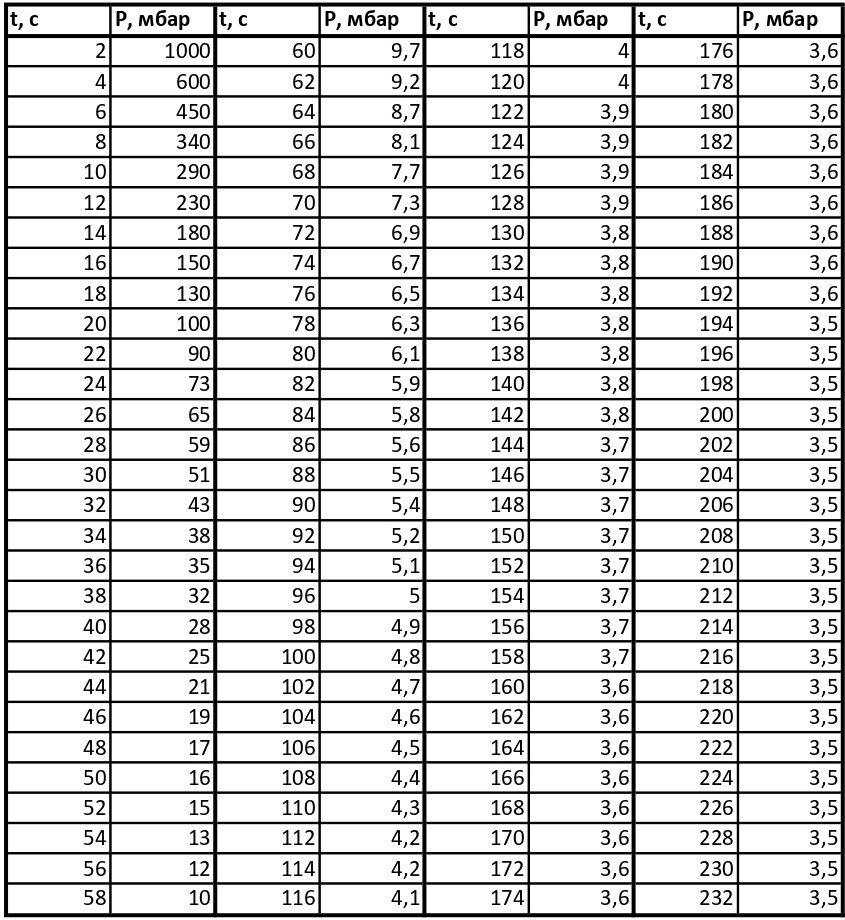
\includegraphics[width = 8cm, height = 8cm]{Диффузный насос, PPT 100_pages-to-jpg-0001.jpg}
  
    \newpage 
    \noindent\textbf{Рисунок 1.} График к таблице 1.
    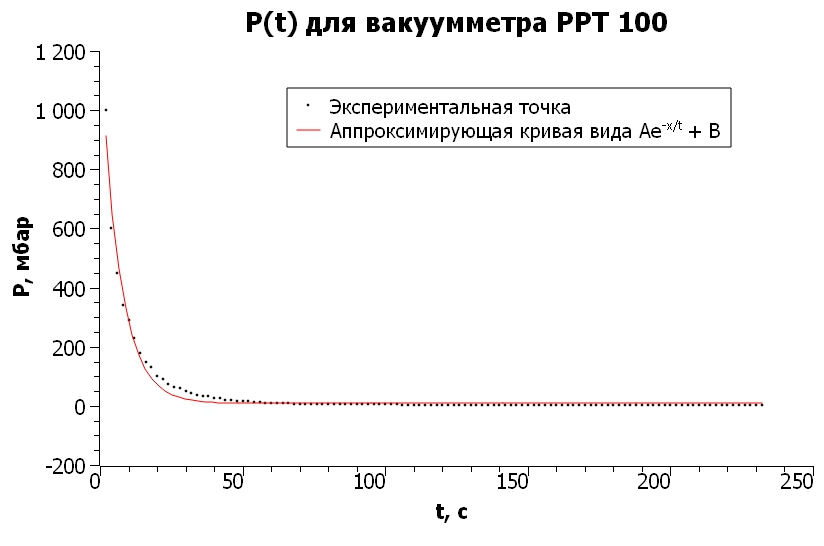
\includegraphics[width = 11cm, height = 7cm]{Диффузный насос, PPT 100.jpg}
    
    \newpage
    \noindent\textbf{Таблица 2.} Зависимость давления от времени откачки диффузным насосом по данным вакуумметра MPT 100.
    
    \centering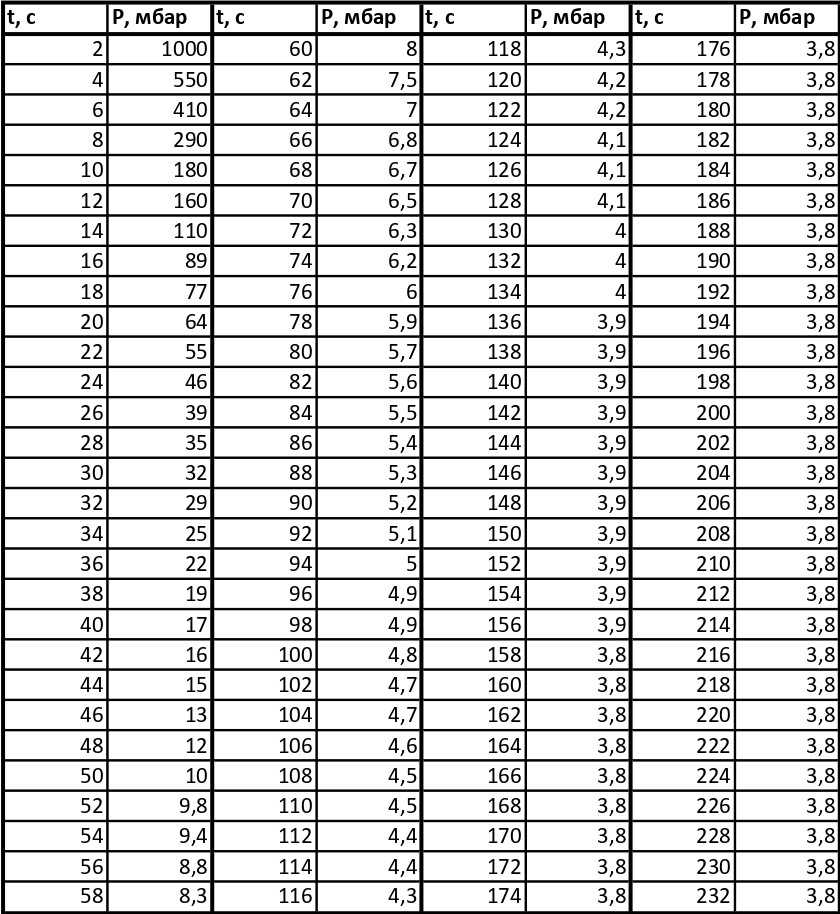
\includegraphics[width = 8cm, height = 8cm]{Диффузный насос, MPT 100_page-0001.jpg}
    
    \newpage
    \noindent\textbf{Рисунок 2.} График к таблице 2.
    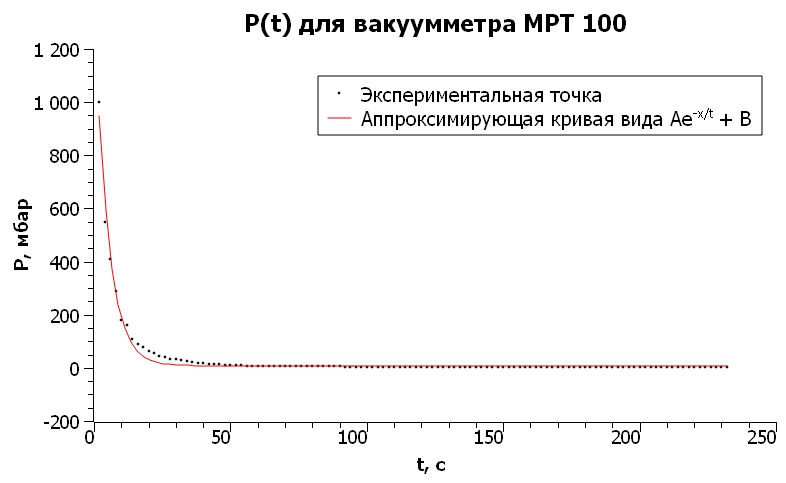
\includegraphics[width = 11cm, height = 7cm]{Диффузный насос, MPT 100.jpg}
    
    \newpage
    \noindent\textbf{Таблица 3.} Зависимость давления от времени откачки турбомолекулярным насосом по данным вакуумметра PPT 100.
    
    \centering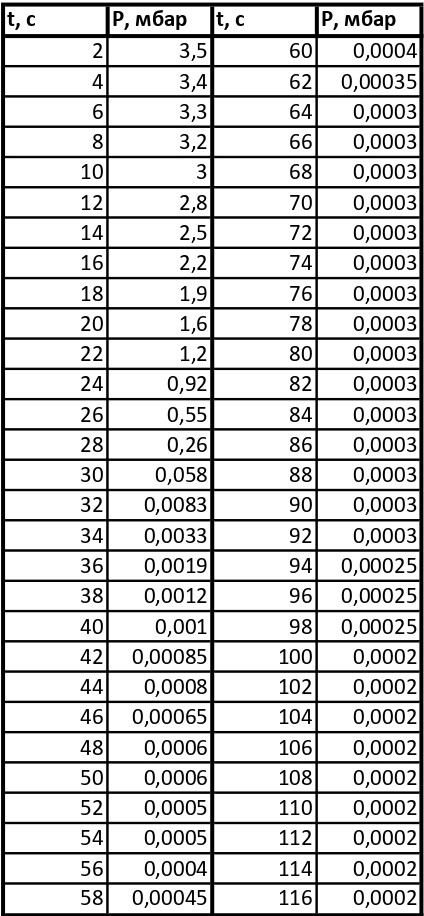
\includegraphics[width = 8cm, height = 15cm]{Турбомолекулярный насос, PPT 100_page-0001.jpg}
    
    \newpage
    \noindent\textbf{Рисунок 3.} График к таблице 3.
    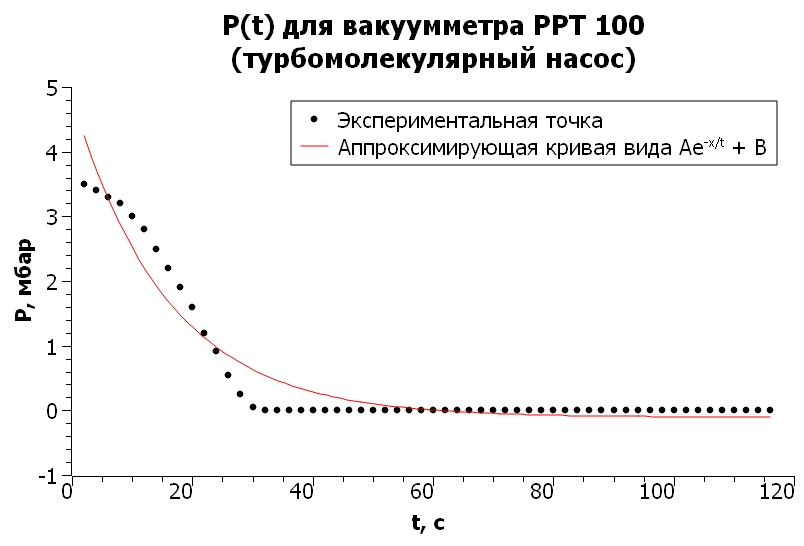
\includegraphics[width = 11cm, height = 7cm]{Турбомолекулярный насос, PPT 100.jpg}
    
    \newpage
    \noindent\textbf{Таблица 4.} Зависимость давления от времени после создания течи по данным вакуумметра PPT 100.
    
    \centering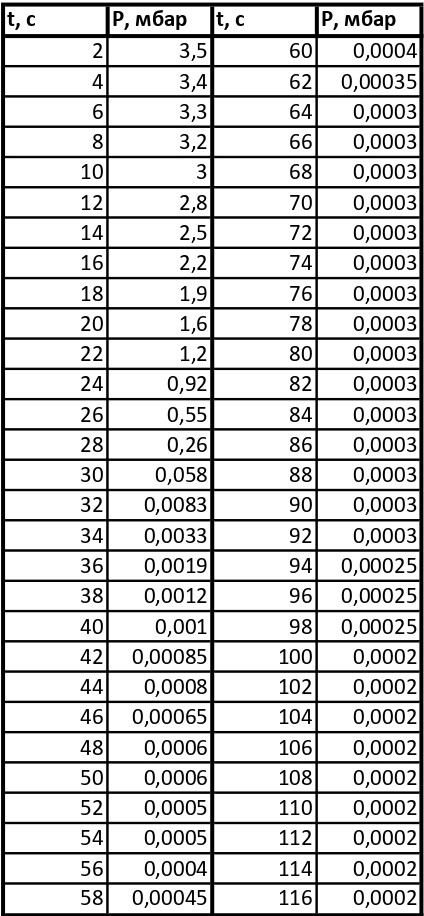
\includegraphics[width = 8cm, height = 15cm]{Турбомолекулярный насос, PPT 100_page-0001.jpg}
    
    \newpage
    \noindent\textbf{Рисунок 4.} График к таблице 4.
    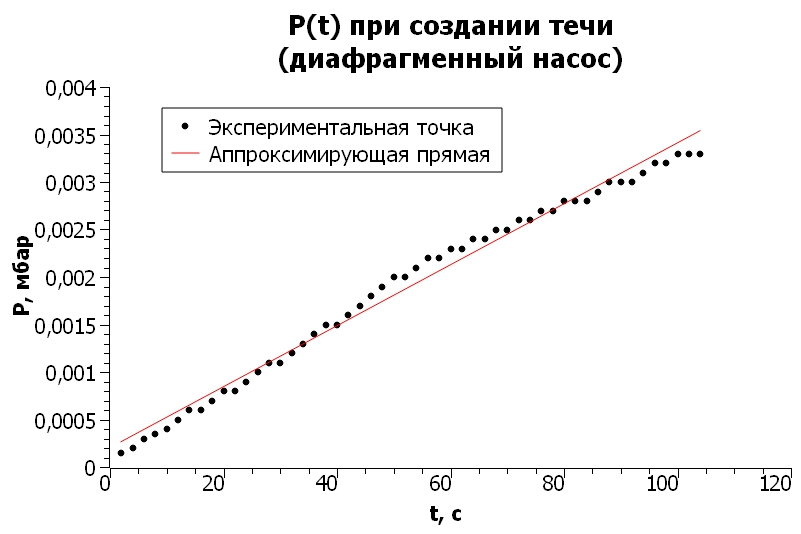
\includegraphics[width = 11cm, height = 7cm]{Течь, PPT 100.jpg}


\end{document}